Physically, a \gls{qcm} is manifest as a thin disc of crystalline quartz,
\ce{SiO2}, with metal electrodes deposited on either side
(\Figure{fig:qcmholding}).  The crystalline structure is specifically
$\alpha$-quartz, organized in a trigonal system which is piezoelectric.
Typically the crystal employs the ``AT-cut'' at an angle of
\SI{35.25}{\degree} with respect to the crystallographic axis.  In the
AT-cut, the vibrational state is dominated by the thickness shear mode,
setting up transverse shear waves along the faces of the crystal
(\Figure{fig:qcmshearwave}).  The AT-cut quartz also has the convenience of
a zero frequency temperature coefficient $df/dT=0$ at \SI{25}{\celsius}.

When an object is deposited on the crystal surface, the surface acoustic
waves will interact with a sample and the resonance frequency of the hybrid
system will change.  This is the principle of \gls{qcm} sensing.
\begin{figure}[t]
 \centering
 	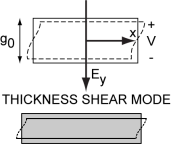
\includegraphics[keepaspectratio]{qcm/figures/qcm_shearmode.pdf}
	\caption{Conceptual drawing of a transverse shear wave.  An electric
	potential is applied along the $y$ axis, causing the crystal to
	shear.}
\label{fig:qcmshearwave}
\end{figure}
